\chapter{Homology}
\section{Simplicial Complexes}
An $n$-Simplex is an set of $(n+1)$ linearly independent points. We can think of them as $n$-dimensional generalizations of triangles.

For some low dimensional examples,
\begin{center}
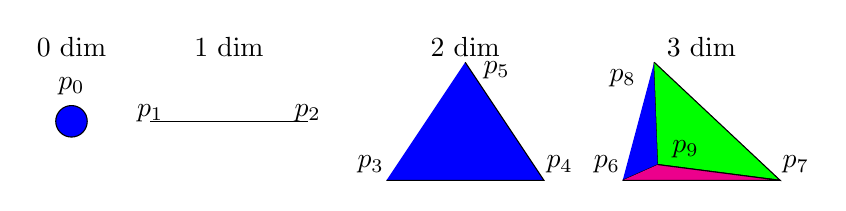
\begin{tikzpicture}
  \draw[fill=blue] (0,.75) circle (0.2);
  \draw (0,1.2) node{ $p_0$};
  \draw (0,1.7) node{0 dim};

  \draw (1,.75) -- (3,.75);
  \draw (1,.85) node{$p_1$};
  \draw (3,.85) node{$p_2$};
  \draw (2,1.7) node{1 dim};

  \draw[fill=blue] (4,0) -- (6,0) -- (5,1.5);
  \draw (3.8,.2) node{$p_3$};
  \draw (6.2,.2) node{$p_4$};
  \draw (5.4,1.4) node{$p_5$};
  \draw (5,1.7) node{2 dim};

  \draw[fill=blue] (7,0) -- (7.45,.2) -- (7.4,1.5);
  \draw[fill=green] (7.45,.2) -- (9,0) -- (7.4,1.5);
  \draw[fill=magenta] (7,0) -- (9,0) -- (7.45,.2);
  \draw (6.8,.2) node{$p_6$};
  \draw (9.2,.2) node{$p_7$};
  \draw (7,1.3) node{$p_8$};
  \draw (7.8,.4) node{$p_9$};
  \draw (8,1.7) node{3 dim};

\end{tikzpicture}
\end{center}

Both unoriented and oriented simplices exist.  For our purposes, we will be using oriented simplices.  The orietnation is a positive or negative sign associated with the set.  Permuting the order of the points in the set can change the orientation.
\begin{equation}
  p_1 p_2 = - p_2 p_1 \qquad \qquad p_3 p_4 p_5 = - p_4 p_3 p_5 = p_5 p_3 p_4
\end{equation}
\begin{center}
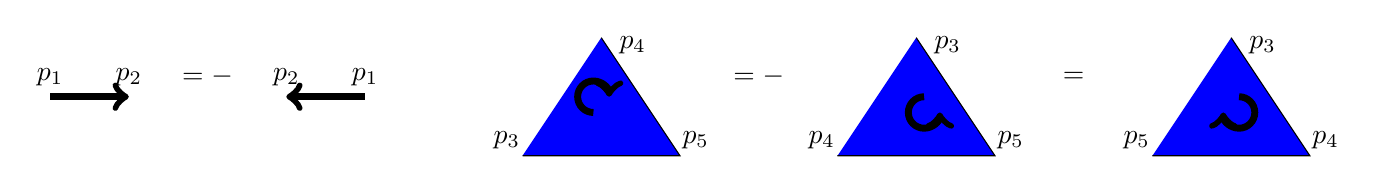
\begin{tikzpicture}
  \draw[->,line width=2.5] (1,.75) -- (2,.75);
  \draw (1,1) node{$p_1$};
  \draw (2,1) node{$p_2$};

  \draw (3,1) node{$=-$};

  \draw[<-,line width=2.5] (4,.75) -- (5,.75);
  \draw (4,1) node{$p_2$};
  \draw (5,1) node{$p_1$};


  \draw[fill=blue] (7,0) -- (9,0) -- (8,1.5);
  \draw (6.8,.2) node{$p_3$};
  \draw (9.2,.2) node{$p_5$};
  \draw (8.4,1.4) node{$p_4$};
  \draw[line width=2.5,<-] (8.1,.75) arc(0:270:.2);

  \draw (10,1) node{$=-$};

  \draw[fill=blue] (11,0) -- (13,0) -- (12,1.5);
  \draw (10.8,.2) node{$p_4$};
  \draw (13.2,.2) node{$p_5$};
  \draw (12.4,1.4) node{$p_3$};
  \draw[line width=2.5,->] (12.1,.75) arc(90:360:.2);

  \draw (14,1) node{$=$};

  \draw[fill=blue] (15,0) -- (17,0) -- (16,1.5);
  \draw (14.8,.2) node{$p_5$};
  \draw (17.2,.2) node{$p_4$};
  \draw (16.4,1.4) node{$p_3$};
  \draw[line width=2.5,->] (16.1,.75) arc(90:-180:.2);

\end{tikzpicture}
\end{center}
While we can see direction in one and two dimensions, this concept is trickier to conceptualize in higher dimensions.  In higher dimensions, instead of thinking pictorially, we need to just think in terms of even or odd permutations of an ordered set.
\begin{equation}
  p_1 p_2 p_3 p_4 p_5 = - (p_2 p_1) p_3 p_4 p_5
\end{equation}

By adding multiple simplices of the same dimension together, we can form a \textbf{chain}.  For example, this is a 2-chain,
\begin{equation}
  p_1 p_2 p_2 + p_2 p_3 p_4
\end{equation}
\begin{center}
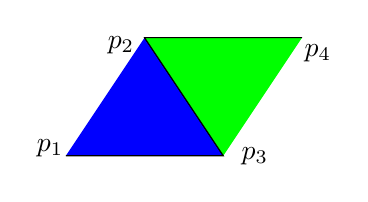
\begin{tikzpicture}
  \draw (-.2,.1) node{$p_1$};
  \draw (.7,1.4) node{$p_2$};
  \draw (2.4,0) node{$p_3$};
  \draw (3.2,1.3) node{$p_4$};

  \draw[fill=blue] (0,0) -- (2,0) -- (1,1.5);
  \draw[fill=green] (2,0) -- (1,1.5) -- (3,1.5);
\end{tikzpicture}
\end{center}

Each simplex gives us a collection of points.  From that collection of points, we can decide to just choose a subset of those and look at those instead.  This subset is a \textbf{face} of the simplex.  For example, if we look at the three dimsional simplex above, $p_6 p_7 p_8 p_9$, we could choose the 2-face $p_6 p_7 p_8$.  All the faces make up the boundaries and edges of an object. We should be able to determine things about the boundaries of an object that are independent of the particular way we write in down but just dependent on the global, qualitative features of the object.  This will show up in how an object relates to its faces.

To study how an object relates to its faces, we need to introduce a boundary operator  $ \partial: \sigma_n \rightarrow \sigma_{n-1} $
\begin{tcolorbox}
\begin{equation}
  \partial \left(p_1 \dots p_n \right)
  = \sum_{i=1}^n (-1)^{i} p_1 \dots \hat{p_i} \dots p_n
\end{equation}
\end{tcolorbox}
where $\hat{p_i}$ is ommitted.  For example,
\begin{align}
  \partial(p_0) &= 0 \\
  \partial(p_1 p_2) & = p_2 - p_1 \\
  \partial(p_1 p_2 p_3) & = -p_2 p_3 + p_1 p_3 - p_1 p_2
\end{align}
The boundary of a boundary is always zero,
\begin{tcolorbox}
  \begin{equation}\label{eq:boundary_zero}
    \partial \partial \sigma =0.
  \end{equation}
\end{tcolorbox}
We can verify this for the boundaries just calculated,
\begin{align}
  \partial \partial (p_0 )& = \partial 0  &= 0 \\
  \partial \partial (p_1 p_2 )&= \partial (p_2 - p_1) &= 0 \\
  \partial \partial (p_1 p_2 p_3 )&= \partial (-p_2 p_3 + p_1 p_3 - p_1 p_2) &=
    p_2 - p_3 -p_1 + p_3  + p_1 -p_2 =0 ,
\end{align}
or in general for any dimension.





\begin{definition}[Simplicial Complex]
  A simplicial complex is a set of of simplices $\kappa$ such that
  \begin{itemize}
    \item For every simplex $\sigma \in \kappa$, every face of the simplex is also in $\kappa$
    \item The intersection of two simplices is a face of both simplces, $\sigma_1 \cap \sigma_2 \in \sigma_1 , \sigma_2$
  \end{itemize}
\end{definition}

For example,
\begin{center}
  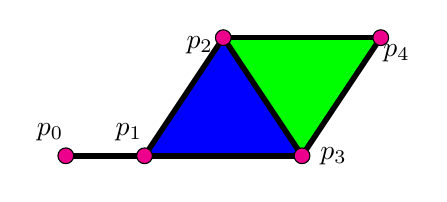
\begin{tikzpicture}

    \draw[fill=blue] (0,0) -- (2,0) -- (1,1.5);
    \draw[fill=green] (2,0) -- (1,1.5) -- (3,1.5);

    \draw[line width=2] (0,0) -- (-1,0);
    \draw[line width=2] (0,0) -- (1,1.5);
    \draw[line width=2] (0,0) -- (2,0);
    \draw[line width=2] (2,0) -- (1,1.5);
    \draw[line width=2] (1,1.5) -- (3,1.5);
    \draw[line width=2] (2,0) -- (3,1.5);

    \draw  (-1.2,.3) node{$p_0$};
    \draw[fill=magenta] (-1,0) circle (0.1);
    \draw (-.2,.3) node{$p_1$};
    \draw[fill=magenta] (0,0) circle (0.1);
    \draw (.7,1.4) node{$p_2$};
    \draw[fill=magenta] (1,1.5) circle (0.1);
    \draw (2.4,0) node{$p_3$};
    \draw[fill=magenta] (2,0) circle (0.1);
    \draw (3.2,1.3) node{$p_4$};
    \draw[fill=magenta] (3,1.5) circle (0.1);

  \end{tikzpicture}
\begin{tabular}{c c c}
  \hline
  dim 0 & dim 1 & dim 2 \\
  \hline
  $p_0$ & $p_0 p_1$ & $p_1 p_2 p_3 $ \\
  $p_1$ & $p_1 p_2$ & $p_2 p_3 p_4 $ \\
  $p_2$ & $p_2 p_3$ & \\
  $p_3$ & $p_3 p_4$ & \\
  $p_4$ & $p_4 p_2$ & \\
   & $p_1 p_3$ & \\
   \hline
\end{tabular}
\end{center}
is a simplicial complex.  If we take the intersection of the simplices $p_1 p_2 p_3$ and $p_2 p_3 p_4$, we get $p_2 p_3$, which is a face of both simplices and in the simplicial complex.

But
\begin{center}
  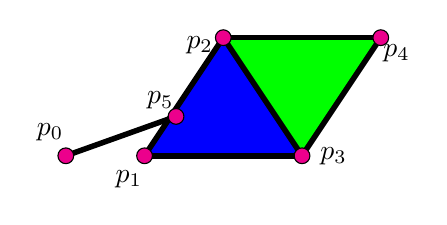
\begin{tikzpicture}

    \draw[fill=blue] (0,0) -- (2,0) -- (1,1.5);
    \draw[fill=green] (2,0) -- (1,1.5) -- (3,1.5);

    \draw[line width=2] (.4,.5) -- (-1,0);

    \draw[line width=2] (0,0) -- (2,0);
    \draw[line width=2] (0,0) -- (1,1.5);
    \draw[line width=2] (2,0) -- (1,1.5);
    \draw[line width=2] (1,1.5) -- (3,1.5);
    \draw[line width=2] (2,0) -- (3,1.5);


    \draw  (-1.2,.3) node{$p_0$};
    \draw[fill=magenta] (-1,0) circle (0.1);
    \draw (-.2,-.3) node{$p_1$};
    \draw[fill=magenta] (0,0) circle (0.1);
    \draw (.7,1.4) node{$p_2$};
    \draw[fill=magenta] (1,1.5) circle (0.1);
    \draw (2.4,0) node{$p_3$};
    \draw[fill=magenta] (2,0) circle (0.1);
    \draw (3.2,1.3) node{$p_4$};
    \draw[fill=magenta] (3,1.5) circle (0.1);

    \draw (.2,.7) node{$p_5$};
    \draw[fill=magenta] (.4,.5) circle (0.1);
  \end{tikzpicture}
\end{center}
is not a simplicial complex.  What even is the intersection of $p_0 p_5$ and $p_1 p_2$?  It's certainly not a face of either simplex.

The simplicial complex
\begin{center}
  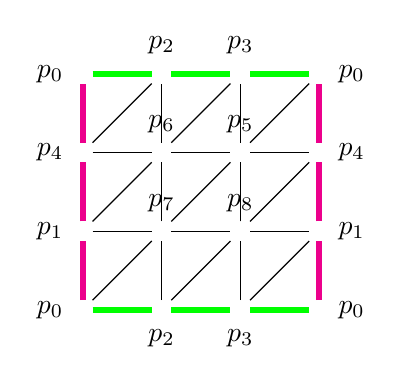
\begin{tikzpicture}
    \node (p0) at (0,0) [label=left:$p_0$]{};
    \node (p1) at (0,1) [label=left:$p_1$]{};
    \node (p2) at (1,0) [label=below:$p_2$]{};
    \node (p3) at (2,0) [label=below:$p_3$]{};
    \node (p4) at (0,2) [label=left:$p_4$]{};

    \node (p7) at (1,1) [label=above:$p_7$]{};
    \node (p8) at (2,1) [label=$p_8$]{};
    \node (p5) at (2,2) [label=$p_5$]{};
    \node (p6) at (1,2) [label=$p_6$]{};

    \node (p0p) at (3,0) [label=right:$p_0$]{};
    \node (p0ppp) at (3,3) [label=right:$p_0$]{};
    \node (p0pp) at (0,3) [label=left:$p_0$]{};
    \node (p1p) at (3,1) [label=right:$p_1$]{};
    \node (p2p) at (1,3) [label=above:$p_2$]{};
    \node (p3p) at (2,3) [label=above:$p_3$]{};
    \node (p4p) at (3,2) [label=right:$p_4$]{};

     \draw[magenta, line width = 2] (p0) -- (p1);
     \draw[magenta, line width = 2] (p0p) -- (p1p);
     \draw[magenta, line width = 2] (p1) -- (p4);
     \draw[magenta, line width = 2] (p1p) -- (p4p);
     \draw[magenta, line width = 2] (p4) -- (p0pp);
     \draw[magenta, line width = 2] (p4p) -- (p0ppp);

     \draw[green, line width = 2] (p0) -- (p2);
     \draw[green, line width = 2] (p2) -- (p3);
     \draw[green, line width = 2] (p3) -- (p0p);
     \draw[green, line width = 2] (p0pp) -- (p2p);
     \draw[green, line width = 2] (p2p) -- (p3p);
     \draw[green, line width = 2] (p3p) -- (p0ppp);

     \draw (p1) -- (p7);
     \draw (p0) -- (p7);
     \draw (p2) -- (p7);

     \draw (p2) -- (p8);
     \draw (p7) -- (p8);
     \draw (p3) -- (p8);

     \draw (p3) -- (p1p);
     \draw (p8) -- (p1p);
     \draw (p8) -- (p4p);
     \draw (p8) -- (p5);

     \draw (p1) -- (p6);
     \draw (p4) -- (p6);
     \draw (p7) -- (p6);

     \draw (p6) -- (p5);
     \draw (p7) -- (p5);
     \draw (p8) -- (p5);

     \draw (p5) -- (p4p);
     \draw (p5) -- (p0ppp);
     \draw (p5) -- (p3p);

     \draw (p6) -- (p3p);
     \draw (p6) -- (p2p);
     \draw (p4) -- (p2p);

  \end{tikzpicture}
\end{center}
is equivalent to a torus.  You can see that that edges are in fact the same points.  Since I couldn't figure out how to perform this manipulation with computer graphics, here's the manipulation with good, old fashioned arts and crafts,

\includegraphics[width=.25\textwidth]{pics/flat_torus.JPG}
{\fontsize{50}{60}\selectfont $\rightarrow$}
\includegraphics[width=.25\textwidth]{pics/torus_1curl.JPG}
{\fontsize{50}{60}\selectfont $\rightarrow$}
\includegraphics[width=.25\textwidth]{pics/torus_2curl.JPG}

I'll often use this simplicial complex as it's relatively simple, yet it still has some interesting structure.

\subsection{The group of cycles and the group of boundaries}

Let's take a chain.  For example,
\begin{equation}
\sigma_1=  p_7 p_6 + p_6 p_5 + p_5 p_7
\end{equation}
in the torus.  Two things about this chain are relevantly interesting to us.  First,
\begin{equation}
  \partial \sigma_1 = 0.
\end{equation}
The boundary of the chain is zero.  You can verify this for yourself.  Second,
\begin{equation}
  \exists \sigma_2 \qquad \text{such that} \qquad \partial \sigma_2 = \sigma_1.
\end{equation}
In particular, $\sigma_2 = p_7 p_6 p_5$, but that fact is not as important as the fact that \textit{it exists}.

The first property defines \textbf{Cycles}.
\begin{definition}[Cycle]
  A \textbf{Cycle} of dimension $d$ is a chain of dimension $d$ $\sigma$ in a simplicial complex such that $\partial \sigma =0$.
\end{definition}
We can add any two cycles of the same dimension together and get another cycle just because the boundary operator is distributive.  This means we have a group, particularly the group $Z_d (T)$, where $T$ is the given topology and $d$ is the dimension.

The second property defines \textbf{Boundaries}.
\begin{definition}[Boundary]
  If $\partial \sigma_2 = \sigma_1$ for some $\sigma_2$, then $\sigma_1$ is a \textbf{boundary}.
\end{definition}
 If a chain is the derivative of something else, then it is a boundary.  More formally, it's the image of the $\partial$ operator.  Boundaries of a certain dimension again will form a group $B_d (T)$, because of the distributivity of the boundary operator.

Since we know from eq~\ref{eq:boundary_zero} that the second derivative of every chain is zero, and every boundary is the derivative of a chain, then the derivative of every boundary is zero. Every boundary is then.... you guessed it... I hope, or I failed in explaining this ... a cycle.

\textbf{BUT} not every cycle is a boundary.

To see this, let us go back to our trusty torus and look at the cycle
\begin{equation}\label{eq:not_boundary}
  p_1 p_7 + p_7 p_8 + p_8 p_1.
\end{equation}
Go ahead an verify that this is indeed a cycle.  That is a rather straight forward calculation.  And then, waste some period of time trying to find a combination of simplices that will give that particular chain upon derivation.  Then give up and say it's impossible.  Physicist's proof.

You can think of every boundary being able to be continuously deformed to a point through the surface that it borders. But the chain~\ref{eq:not_boundary} can't be deformed away to a point because it wraps around the torus.  Only cutting and glueing the torus would allow you to deform that cycle down into a point.

  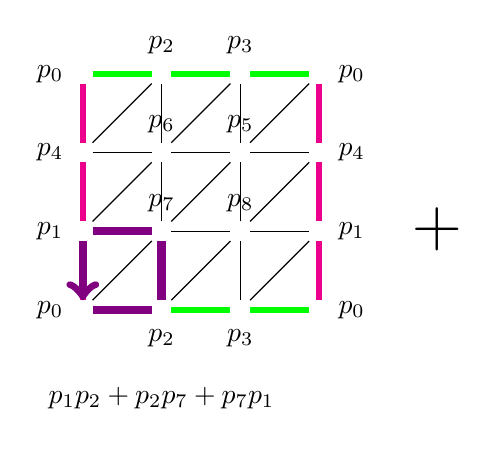
\begin{tikzpicture}
    \node (p0) at (0,0) [label=left:$p_0$]{};
    \node (p1) at (0,1) [label=left:$p_1$]{};
    \node (p2) at (1,0) [label=below:$p_2$]{};
    \node (p3) at (2,0) [label=below:$p_3$]{};
    \node (p4) at (0,2) [label=left:$p_4$]{};

    \node (p7) at (1,1) [label=above:$p_7$]{};
    \node (p8) at (2,1) [label=$p_8$]{};
    \node (p5) at (2,2) [label=$p_5$]{};
    \node (p6) at (1,2) [label=$p_6$]{};

    \node (p0p) at (3,0) [label=right:$p_0$]{};
    \node (p0ppp) at (3,3) [label=right:$p_0$]{};
    \node (p0pp) at (0,3) [label=left:$p_0$]{};
    \node (p1p) at (3,1) [label=right:$p_1$]{};
    \node (p2p) at (1,3) [label=above:$p_2$]{};
    \node (p3p) at (2,3) [label=above:$p_3$]{};
    \node (p4p) at (3,2) [label=right:$p_4$]{};

     \draw[magenta, line width = 2] (p0) -- (p1);
     \draw[magenta, line width = 2] (p0p) -- (p1p);
     \draw[magenta, line width = 2] (p1) -- (p4);
     \draw[magenta, line width = 2] (p1p) -- (p4p);
     \draw[magenta, line width = 2] (p4) -- (p0pp);
     \draw[magenta, line width = 2] (p4p) -- (p0ppp);

     \draw[green, line width = 2] (p0) -- (p2);
     \draw[green, line width = 2] (p2) -- (p3);
     \draw[green, line width = 2] (p3) -- (p0p);
     \draw[green, line width = 2] (p0pp) -- (p2p);
     \draw[green, line width = 2] (p2p) -- (p3p);
     \draw[green, line width = 2] (p3p) -- (p0ppp);

     \draw (p1) -- (p7);
     \draw (p0) -- (p7);
     \draw (p2) -- (p7);

     \draw (p2) -- (p8);
     \draw (p7) -- (p8);
     \draw (p3) -- (p8);

     \draw (p3) -- (p1p);
     \draw (p8) -- (p1p);
     \draw (p8) -- (p4p);
     \draw (p8) -- (p5);

     \draw (p1) -- (p6);
     \draw (p4) -- (p6);
     \draw (p7) -- (p6);

     \draw (p6) -- (p5);
     \draw (p7) -- (p5);
     \draw (p8) -- (p5);

     \draw (p5) -- (p4p);
     \draw (p5) -- (p0ppp);
     \draw (p5) -- (p3p);

     \draw (p6) -- (p3p);
     \draw (p6) -- (p2p);
     \draw (p4) -- (p2p);

     \draw[violet, line width=3, ->] (p0) -- (p2) -- (p7) -- (p1) -- (p0);

     \node (text) at (4.5,.5) [label={\fontsize{30}{40}\selectfont$+$}]{};
     \draw (text);

     \node (name) at (1,-1.5) [label=$p_1 p_2+p_2 p_7 + p_7 p_1$]{};
     \draw (text);
  \end{tikzpicture}
  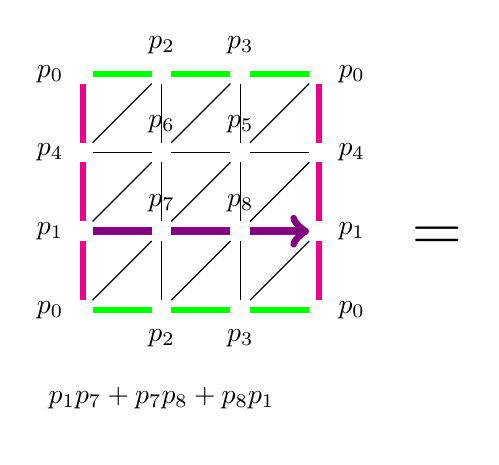
\begin{tikzpicture}
    \node (p0) at (0,0) [label=left:$p_0$]{};
    \node (p1) at (0,1) [label=left:$p_1$]{};
    \node (p2) at (1,0) [label=below:$p_2$]{};
    \node (p3) at (2,0) [label=below:$p_3$]{};
    \node (p4) at (0,2) [label=left:$p_4$]{};

    \node (p7) at (1,1) [label=above:$p_7$]{};
    \node (p8) at (2,1) [label=$p_8$]{};
    \node (p5) at (2,2) [label=$p_5$]{};
    \node (p6) at (1,2) [label=$p_6$]{};

    \node (p0p) at (3,0) [label=right:$p_0$]{};
    \node (p0ppp) at (3,3) [label=right:$p_0$]{};
    \node (p0pp) at (0,3) [label=left:$p_0$]{};
    \node (p1p) at (3,1) [label=right:$p_1$]{};
    \node (p2p) at (1,3) [label=above:$p_2$]{};
    \node (p3p) at (2,3) [label=above:$p_3$]{};
    \node (p4p) at (3,2) [label=right:$p_4$]{};

     \draw[magenta, line width = 2] (p0) -- (p1);
     \draw[magenta, line width = 2] (p0p) -- (p1p);
     \draw[magenta, line width = 2] (p1) -- (p4);
     \draw[magenta, line width = 2] (p1p) -- (p4p);
     \draw[magenta, line width = 2] (p4) -- (p0pp);
     \draw[magenta, line width = 2] (p4p) -- (p0ppp);

     \draw[green, line width = 2] (p0) -- (p2);
     \draw[green, line width = 2] (p2) -- (p3);
     \draw[green, line width = 2] (p3) -- (p0p);
     \draw[green, line width = 2] (p0pp) -- (p2p);
     \draw[green, line width = 2] (p2p) -- (p3p);
     \draw[green, line width = 2] (p3p) -- (p0ppp);

     \draw (p1) -- (p7);
     \draw (p0) -- (p7);
     \draw (p2) -- (p7);

     \draw (p2) -- (p8);
     \draw (p7) -- (p8);
     \draw (p3) -- (p8);

     \draw (p3) -- (p1p);
     \draw (p8) -- (p1p);
     \draw (p8) -- (p4p);
     \draw (p8) -- (p5);

     \draw (p1) -- (p6);
     \draw (p4) -- (p6);
     \draw (p7) -- (p6);

     \draw (p6) -- (p5);
     \draw (p7) -- (p5);
     \draw (p8) -- (p5);

     \draw (p5) -- (p4p);
     \draw (p5) -- (p0ppp);
     \draw (p5) -- (p3p);

     \draw (p6) -- (p3p);
     \draw (p6) -- (p2p);
     \draw (p4) -- (p2p);

     \draw[violet, line width=3, ->] (p1) -- (p7) -- (p8)  -- (p1p);

     \node (text) at (4.5,.5) [label={\fontsize{30}{40}\selectfont$=$}]{};
     \draw (text);

     \node (name) at (1,-1.5) [label=$p_1 p_7 + p_7 p_8 + p_8 p_1$]{};
     \draw (text);
  \end{tikzpicture}
  \begin{tikzpicture}
    \node (p0) at (0,0) [label=left:$p_0$]{};
    \node (p1) at (0,1) [label=left:$p_1$]{};
    \node (p2) at (1,0) [label=below:$p_2$]{};
    \node (p3) at (2,0) [label=below:$p_3$]{};
    \node (p4) at (0,2) [label=left:$p_4$]{};

    \node (p7) at (1,1) [label=above:$p_7$]{};
    \node (p8) at (2,1) [label=$p_8$]{};
    \node (p5) at (2,2) [label=$p_5$]{};
    \node (p6) at (1,2) [label=$p_6$]{};

    \node (p0p) at (3,0) [label=right:$p_0$]{};
    \node (p0ppp) at (3,3) [label=right:$p_0$]{};
    \node (p0pp) at (0,3) [label=left:$p_0$]{};
    \node (p1p) at (3,1) [label=right:$p_1$]{};
    \node (p2p) at (1,3) [label=above:$p_2$]{};
    \node (p3p) at (2,3) [label=above:$p_3$]{};
    \node (p4p) at (3,2) [label=right:$p_4$]{};

     \draw[magenta, line width = 2] (p0) -- (p1);
     \draw[magenta, line width = 2] (p0p) -- (p1p);
     \draw[magenta, line width = 2] (p1) -- (p4);
     \draw[magenta, line width = 2] (p1p) -- (p4p);
     \draw[magenta, line width = 2] (p4) -- (p0pp);
     \draw[magenta, line width = 2] (p4p) -- (p0ppp);

     \draw[green, line width = 2] (p0) -- (p2);
     \draw[green, line width = 2] (p2) -- (p3);
     \draw[green, line width = 2] (p3) -- (p0p);
     \draw[green, line width = 2] (p0pp) -- (p2p);
     \draw[green, line width = 2] (p2p) -- (p3p);
     \draw[green, line width = 2] (p3p) -- (p0ppp);

     \draw (p1) -- (p7);
     \draw (p0) -- (p7);
     \draw (p2) -- (p7);

     \draw (p2) -- (p8);
     \draw (p7) -- (p8);
     \draw (p3) -- (p8);

     \draw (p3) -- (p1p);
     \draw (p8) -- (p1p);
     \draw (p8) -- (p4p);
     \draw (p8) -- (p5);

     \draw (p1) -- (p6);
     \draw (p4) -- (p6);
     \draw (p7) -- (p6);

     \draw (p6) -- (p5);
     \draw (p7) -- (p5);
     \draw (p8) -- (p5);

     \draw (p5) -- (p4p);
     \draw (p5) -- (p0ppp);
     \draw (p5) -- (p3p);

     \draw (p6) -- (p3p);
     \draw (p6) -- (p2p);
     \draw (p4) -- (p2p);

     \draw[violet, line width=3, ->] (p1) -- (p0) -- (p2) -- (p7) -- (p8) -- (p1p);

     \node (name) at (1,-1.5) [label=$p_1 p_0 + p_0 p_2 + p_0 p_7 + p_7 p_8 + p_8 p_1$]{};
     \draw (text);
  \end{tikzpicture}



  \begin{equation}
    \left( p_1 p_2+p_2 p_7 + \cancel{p_7 p_1} \right) + \left( \cancel{p_1 p_7} + p_7 p_8 + p_8 p_1 \right)
  \end{equation}


  \begin{equation}
    \partial \left( p_7 p_0 p_1 + p_2 p_0 p_7 \right)
    =  - p_0 p_1 + p_7 p_1 - \cancel{p_7 p_0} - \cancel{p_0 p_7} + p_2 p_7 - p_2 p_0
    = p_0 p_2 + p_2 p_7 + p_7 p_1 + p_1 p_0
  \end{equation}
